\documentclass[12pt]{exam}

\usepackage{amssymb}
\usepackage{mathtools}
\usepackage{algorithm}
\usepackage{float}  % Figure placement
\usepackage{minted}  % Code highlighting
\usepackage{tikz}  % Flow chart
\usepackage{lipsum}
\usepackage{xspace}
\usepackage{hyperref}
\usepackage{MnSymbol}
\usepackage{pgffor}
\usepackage{colortbl}
\usepackage{multirow}
\usepackage{array}


\hypersetup{
    colorlinks = true,
    linkcolor = blue,
    urlcolor  = blue,
    citecolor = blue,
    anchorcolor = blue
}

\newcommand{\hwheaderfooter}[3]{
\pagestyle{headandfoot}
\firstpageheadrule
\firstpageheader{#1}{#2}{#3}
\runningheader{#1}{#2}{#3}
\runningheadrule
\firstpagefooter{}{\thepage}{}
\runningfooter{}{\thepage}{}
}

\newcommand{\latex}{\LaTeX\xspace}

\newcommand{\stars}[1]{%
    \foreach \n in {1,...,#1}{%
        $\filledstar$%
    }%
}

\hwheaderfooter{Ching}{HW 9 Part 2}{CSCI 406}


\begin{document}
\begin{center}
    \fbox{\fbox{\parbox{\textwidth - 0.2 in}{\centering

                {Instructions: Please note that handwritten assignments \textbf{will not be graded}. Use the
                    provided \latex template to complete your homework. Please do not alter the order or spacing of
                    questions (keep each question on its own page). When you submit to Gradescope, you must mark
                    which page(s) correspond to each question. \textbf{You may not receive credit for unmarked
                        questions}. \\ When including graphical figures, we encourage the use of tools such as \href{https://dreampuf.github.io/GraphvizOnline/}{graphviz} or packages like \href{https://www.overleaf.com/learn/latex/TikZ_package}{tikz} for simple and complex figures. However, these may be handwritten only if they are neat and legible (as defined by the grader). }
            }}}
\end{center}

\textbf{List any collaborators (besides TAs or professors) here:}

\begin{questions}

    \question[5] [W12, \stars{1}] NP-Completeness. For the following questions, select whether the statement is true or false,
    and write a \textit{brief} explanation of your reasoning.

    \begin{parts}
        \part Consider two decision problems $A$ and $B$ where $A$ is known to be NP-Complete, and every instance of $B$ can be reduced to an instance of $A$ in polynomial size and time. $B$ is NP-Complete.

        $\blacksquare$ True $\square$ False

        If $A$ is NP-Complete, and $B$ can be reduced to $A$ in polynomial time, then $B$ is also NP-Complete.

        \part If a problem, $X$, is NP-Complete, it is unsolvable

        $\square$ True $\blacksquare$ False

        NP-Complete problems are solvable, but they are not solvable in polynomial time.

        \part Let $\propto$ denote a polynomial-time reduction.
        Then, for problems $X$, $Y$ and $Z$,
        \[
            (X \propto Y) \land (Y \propto Z) \rightarrow (X \propto Z).
        \]
        In other words, the polynomial-time reduction property is transitive

        $\blacksquare$ True $\square$ False

        If $X$ can be reduced to $Y$ in polynomial time, and $Y$ can be reduced to $Z$ in polynomial time, then $X$ can be reduced to $Z$ in polynomial time.

    \end{parts}
    \clearpage

    \question[10] [W12, \stars{3}] Satisfiability. Provide a set of boolean assignments which will satisfy the following expression:
    \[
        (x_1 \lor x_2 \lor x_3) \land
        (x_2 \lor \neg x_3 \lor x_4 \lor \neg x_5) \land
        (\neg x_1 \lor \neg x_5) \land
        (x_3 \lor \neg x_5) \land
        (x_3 \lor x_5) \land
        (\neg x_3 \lor \neg x_4) \land
        (\neg x_2 \lor x_4 \lor x_5)
    \]

    \begin{parts}
        \part $x_1$: $\square$ True $\blacksquare$ False
        \part $x_2$: $\square$ True $\blacksquare$ False
        \part $x_3$: $\blacksquare$ True $\square$ False
        \part $x_4$: $\square$ True $\blacksquare$ False
        \part $x_5$: $\square$ True $\blacksquare$ False
    \end{parts}
    \clearpage

    \question[10] [W12, \stars{3}] Vertex Cover. Indicate which vertices are needed in the optimal vertex cover for the following graph.

    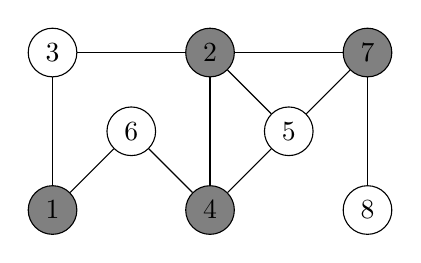
\begin{tikzpicture}
        \node[circle, draw, fill=gray] (1) at (0,0) {1};
        \node[circle, draw, fill=gray] (2) at (2,2) {2};
        \node[circle, draw] (3) at (0,2) {3};
        \node[circle, draw, fill=gray] (4) at (2,0) {4};
        \node[circle, draw] (5) at (3,1) {5};
        \node[circle, draw] (6) at (1,1) {6};
        \node[circle, draw, fill=gray] (7) at (4,2) {7};
        \node[circle, draw] (8) at (4,0) {8};

        \draw (1) -- (3);
        \draw (1) -- (6);
        \draw (2) -- (4);
        \draw (2) -- (3);
        \draw (4) -- (6);
        \draw (4) -- (5);
        \draw (2) -- (7);
        \draw (2) -- (5);
        \draw (5) -- (7);
        \draw (7) -- (8);
    \end{tikzpicture}

    \begin{parts}
        \part 1: $\blacksquare$ Included
        \part 2: $\blacksquare$ Included
        \part 3: $\square$ Included
        \part 4: $\blacksquare$ Included
        \part 5: $\square$ Included
        \part 6: $\square$ Included
        \part 7: $\blacksquare$ Included
    \end{parts}

    \clearpage

    \question[10] [W12, \stars{1}] Satisfiability. Bill has an $n$-SAT problem with 10 clauses that he wishes to reduce to 3-SAT. His instance has:

    \begin{itemize}
        \item 1 one-literal clause
        \item 2 two-literal clauses
        \item 3 four-literal clauses
        \item 4 five-literal clauses
    \end{itemize}

    \begin{parts}
        \part[5] Using the reduction discussed in class, how many clauses will Bill end up with?

        $\boxed{\text{12}}$

        \part[5] Assuming Bill doesn't reuse dummy variables, how many dummy variables will Bill add?

        $\boxed{\text{6}}$

    \end{parts}


    \begin{table}[H]
        \centering
        \begin{tabular}{c|c|c|c}
            \# of literals, k & \# of clauses & new dummy var    & \# 3-literal clause \\
            \hline
            1                 & 1             & 2                & 4                   \\
            2                 & 2             & $1 \times 2 = 2$ & $2 \times 2 = 4 $   \\
            4                 & 3             & 0                & 1                   \\
            5                 & 4             & $(5-3) = 2   $   & $ (5-2) = 3 $       \\ \hline
            total             & 10            & 6                & 12
        \end{tabular}
    \end{table}


    % close the document
\end{questions}
\end{document}
